\documentclass[12pt,letterpaper]{article}
\usepackage{amsmath,amsthm,amsfonts,amssymb,amscd}
\usepackage{listings}
\usepackage{color}
\usepackage{MnSymbol,wasysym}
\usepackage{caption}
\usepackage{subcaption}
\definecolor{codegreen}{rgb}{0,0.6,0}
\definecolor{codegray}{rgb}{0.5,0.5,0.5}
\definecolor{codepurple}{rgb}{0.58,0,0.82}
\definecolor{backcolour}{rgb}{0.95,0.95,0.92}
\definecolor{dkgreen}{rgb}{0,0.6,0}
\definecolor{gray}{rgb}{0.5,0.5,0.5}
\definecolor{mauve}{rgb}{0.58,0,0.82}

\usepackage{biblatex}

\addbibresource{bibliography.bib}

\lstdefinestyle{mystyle}{
  language=R,
  backgroundcolor=\color{backcolour},   commentstyle=\color{codegreen},
  aboveskip=3mm,
  belowskip=3mm,
  showstringspaces=false,
  columns=flexible,
  basicstyle={\small\ttfamily},
  numbers=left,
  numbersep=5pt,
  numberstyle=\tiny\color{gray},
  keywordstyle=\color{blue},
  commentstyle=\color{dkgreen},
  stringstyle=\color{mauve},
  breaklines=true,
  breakatwhitespace=true
  tabsize=2
}

\lstset{style=mystyle}
\usepackage{hyperref}
\usepackage{graphicx}
\usepackage{enumerate}
\usepackage{fancyhdr}
\usepackage{mathrsfs}
\usepackage[margin=3cm]{geometry}
\setlength{\parindent}{0.0in}
\setlength{\parskip}{0.05in}

% Edit these as appropriate
\newcommand\course{CS432}
\newcommand\semester{Spring 2016}     
\newcommand\hwnum{7}
\newcommand\yourname{Kevin R. Clemmons}
\newcommand\login{oduprogrammer16}

\newenvironment{answer}[1]{
  \subsubsection*{Problem #1}
}

\pagestyle{fancyplain}
\headheight 40pt
\lhead{\yourname\ \\(\login)\\\course\ --- \semester}
\chead{\textbf{\Large Assignment \hwnum}}
\rhead{\today}
\headsep 40pt

\begin{document}

All files mentioned in this file are uploaded into the {\it github} repository.

The \LaTeX code invovled in the generation of this document was aided by the example code provided in the links that Dr. Nelson sent out on January 17, 2016 \\ %\cite{mohammedaturban2013}. 

This document was compiled on \url{www.sharelatex.com} \\ \\ 

This assignment utilizes the movie lens data-set to answer the following problems below\cite{grouplens2016,fmaxwellharperjosephakonstan2015}. The data set is contained in a class which utilizes threading to parse all three data-files concurrently. This allows the user to pass in a single variable that functions can use and manipulate the data. 

\begin{answer}{1}
To determine which users are closest to me in terms of characteristics, a program called subsituteYou was written and takes in three command line parameters for my age, gender and occupation. The program searches for users who have the same age, gender and occupation as I do and them prints their ids along with their top three favorite movies and their bottom three least favorite movies along with the rating.

Tables 1, 2 and 3 shows the results produced by the program.  

\begin{table}[ht!]
    \centering
    \begin{tabular}{|c|c|c||c|c|}\hline
    \textbf{Rank} & \textbf{Top Favorite Movies} & \textbf{Rating}  & \textbf{Least Favorite Films} & \textbf{Rating}\\ \hline
     1 & Titanic (1997) & 5.0 & Liar Liar (1997) & 3.0 \\\hline 
     2 & Game, The (1997) & 4.0 & Soul Food (1997) & 3.0 \\\hline 
     3 & Air Force One (1997) & 4.0 & Devil's Own, The (1997) & 3.0 \\\hline 
    \end{tabular}
    \caption{Movie recommendations for user 33}
    \label{tab:my_label}
\end{table}

\begin{table}[ht!]
    \centering
    \begin{tabular}{|c|c|c||c|c|}\hline
    \textbf{Rank} & \textbf{Top Favorite Movies} & \textbf{Rating}  & \textbf{Least Favorite Films} & \textbf{Rating}\\ \hline
     1 & Pulp Fiction (1994) & 5.0 & Jurassic Park (1993) & 1.0 \\\hline 
     2 & Raiders of the Lost Ark (1981) & 5.0 & Twister (1996) & 2.0 \\\hline 
     3 & Terminator, The (1984) & 5.0 & Arrival, The (1996) & 2.0 \\\hline 
    \end{tabular}
    \caption{Movie recommendations for user 37}
    \label{tab:my_label}
\end{table}

\begin{table}[ht!]
    \centering
    \begin{tabular}{|c|c|c||c|c|}\hline
    \textbf{Rank} & \textbf{Top Favorite Movies} & \textbf{Rating}  & \textbf{Least Favorite Films} & \textbf{Rating}\\ \hline
     1 & Bringing Up Baby (1938) & 5.0 & Mars Attacks! (1996) & 2.0 \\\hline 
     2 & Toy Story (1995) & 5.0 & Independence Day (ID4) (1996) & 2.0 \\\hline 
     3 & City of Lost Children, The (1995) & 5.0 & Air Force One (1997) & 2.0 \\\hline 
    \end{tabular}
    \caption{Movie recommendations for user 838}
    \label{tab:my_label}
\end{table}

\newpage 
For the ``substitute me'', I will choose user 33. The only major outlier in this user is that I enjoyed the movie Liar Liar. 
\end{answer}
%
\begin{answer}{2}
To determine which users were correlated for the ``substitute me'', a program called correlation-coefficient was written. The program takes in a user id as a command line argument and utilizes a function called simPearson which computes the Pearson correlation coefficient for the ``substitute me'' and the other users in the u.data data-set\cite{tobysegaran2007}. \\

The formula for the pearson correalation-coefficient is computed via the following formula\cite{fmaxwellharperjosephakonstan2015} $\displaystyle r = \frac{\sum XY - \frac{\sum X \sum Y}{N} }{\sqrt{ (\sum X^{2} - \frac{(\sum X)^{2}}{N})(\sum Y^{2} - \frac{(\sum Y)^{2}}{N})}}$. \\  \\ Where $X$ and $Y$ represent ratings for common movies that two people have rated. \\

Listing 1 shows the function that computes the pearson correlation coefficent\cite{fmaxwellharperjosephakonstan2015}. 

\begin{lstlisting}[language=Python, caption=Computing the Pearson Correlation Coefficient]
def sim_Pearson(prefs,p1,p2):
	#This code taken from page 13 in collective intelligence book

	similarItems={}

	for item in prefs[p1]:
		if item in prefs[p2]:
			similarItems[item] = 1

	# Find the number of elements 
	n = len(similarItems)

	# If they have no items in common return 0
	if n == 0:
		return 0

	# Add up all the preferences 
	sum1 = sum([prefs[p1][it] for it in similarItems])
	sum2 = sum([prefs[p2][it] for it in similarItems])

	# Sum up the squares 
	sum1Sq = sum([math.pow(prefs[p1][it],2) for it in similarItems])
	sum2Sq = sum([math.pow(prefs[p2][it],2) for it in similarItems])

	# Sum up the products 
	pSum = sum([prefs[p1][it] * prefs[p2][it] for it in similarItems])

	# Calculate the pearson score 
	num = pSum - (sum1*sum2/n)

	den = math.sqrt((sum1Sq-pow(sum1,2)/n) * (sum2Sq-pow(sum2,2)/n))
	
	# Check if the denominator is zero
	if den == 0:
		return 0
	
	r = num/den

	return r
\end{lstlisting}
Table 4 shows which users had a high and low correlation for the ``substitute me''.
\begin{table}[ht!]
    \centering
    \begin{tabular}{|c|p{3cm}|p{3cm}||c|p{3cm}|}\hline
    \textbf{Rank} & \textbf{Ids with high correlation} & \textbf{Correlation \newline Coefficient}  & \textbf{Ids with low correlation} & \textbf{Correlation Coefficient}\\ \hline
     1 & 890 & +1.0 & 876 & -1.0 \\\hline 
     2 & 718 & +1.0 & 882 & -1.0 \\\hline 
     3 & 937 & +1.0 & 900 & -1.0 \\\hline 
     4 & 22 &  +1.0 & 736 & -1.0 \\\hline 
     5 & 33 &  +1.0 & 657 & -1.0 \\\hline 
    \end{tabular}
    \caption{User Correlation}
    \label{tab:my_label}
\end{table}

It should be noted that in table 4, the correlation coefficients are the same for both the most correlated users and least correlated users. This is due to the number of ratings. 
\end{answer}
%
\newpage
\begin{answer}{3}
To compute ratings for all the films that the ``subsitute me'' has not seen, a program called filmRecomender was created. The program has the ability to take in multiple command line arguments. One of those command line arguments is a flag $-u$ followed by a list of recomended films and a list of films that are not recomended at alol. The program utilizes a function called filmRecomendations which can be seen in listing 2 , utilizes a function called getRecomendations to generate the list of recomended films and sorts the ratings from greatest to least\cite{tobysegaran2007}. 

\begin{lstlisting}[language=Python, caption=Function to get a list of recomended films]
def getRecommendedItems(prefs,itemMatch,user):
  userRatings=prefs[user]
  scores={}
  totalSim={}
  # Loop over items rated by this user
  for (item,rating) in userRatings.items():

    # Loop over items similar to this one
    for (similarity,item2) in itemMatch[item]:

      # Ignore if this user has already rated this item
      if item2 in userRatings: continue
      # Weighted sum of rating times similarity
      scores.setdefault(item2,0)
      scores[item2]+=similarity*rating
      # Sum of all the similarities
      totalSim.setdefault(item2,0)
      totalSim[item2]+=similarity

  # Divide each total score by total weighting to get an average
  rankings=[(score/totalSim[item],item) for item,score in scores.items()]

  # Return the rankings from highest to lowest
  rankings.sort()
  rankings.reverse()

  # Convert tuple to dic

  return rankings
\end{lstlisting}
\newpage 
Tables 5 and 6 show the results of the filmRecomendations. It should be noted the films were randomly selected due to the fact that many of the films had the same ratings.
\begin{table}[ht!]
    \centering
    \begin{tabular}{|c|c|c|}\hline
    \textbf{Rank} & \textbf{Films} & \textbf{Rating} \\ \hline
     1 &  Santa with Muscles (1996) & 5.0 \\\hline 
     2 &  Tough and Deadly (1995) & 5.0 \\\hline 
     3 & Saint of Fort Washington, The (1993) & 5.0 \\\hline 
     4 & Marlene Dietrich: Shadow and Light (1996) &  5.0 \\\hline 
     5 &  Prefontaine (1997) & 5.0 \\\hline 
    \end{tabular}
    \caption{Recommended films for user 33}
    \label{tab:my_label}
\end{table}

\begin{table}[ht!]
    \centering
    \begin{tabular}{|c|c|c|}\hline
    \textbf{Rank} & \textbf{Film} & \textbf{Rating} \\ \hline
     1 & Amityville 1992: It's About Time (1992) & 1.0 \\\hline 
     2 & Children of the Corn: The Gathering (1996) & 1.0 \\\hline 
     3 & 3 Ninjas: High Noon At Mega Mountain (1998) & 1.0 \\\hline 
     4 & Turbo: A Power Rangers Movie (1997) &  1.0 \\\hline 
     5 & Theodore Rex (1995) & 1.0 \\\hline 
    \end{tabular}
    \caption{Films Not Recommended for user 33}
    \label{tab:my_label}
\end{table}
\end{answer}
%
\newpage 
\begin{answer}{4}
To get recommendations based on a certain film, the same code that was used in problem 3 was used. The main difference is that a function called transformPrefs is used to transform the data from the movie perspective\cite{fmaxwellharperjosephakonstan2015}. For this problem, I chose Crimson Tide as my favorite movie and Toy Story. Crimson Tide has movie id number 31 and Batman Forever has movie id number 29. The movie ids are given to the filmRecomender and the recommendations for Crimson Tide are listed below in tables 7 and 8 and the recommendations for Toy Story are listed in tables 9 and 10. \\ \\ 

\begin{center}This space intentionally left blank. } \end{center}

\newpage 
\begin{table}[ht!]
    \centering
    \begin{tabular}{|c|c|c|c|}\hline
    \textbf{Rank} & \textbf{Film} & \textbf{Rating} & \textbf{Like/Dislike}\\ \hline
     1 &  Leave It to Beaver (1997) & 4.84 & Like \\\hline 
     2 & Days of Thunder (1990) & 4.81 & Like \\\hline 
     3 & Sleepers (1996) & 4.80 & Like \\\hline 
     4 & Streetcar Named Desire, A (1951) &  4.70 & Like \\\hline 
     5 & Craft, The (1996) & 4.64 & Like \\\hline 
    \end{tabular}
    \caption{Film Recommendations for Crimson Tide}
    \label{tab:my_label}
\end{table}

\begin{table}[ht!]
    \centering
    \begin{tabular}{|c|c|c|c|}\hline
    \textbf{Rank} & \textbf{Film} & \textbf{Rating} & \textbf{Like/Dislike} \\ \hline
     1 & Body Snatcher, The (1945) & 2.15 & Dislike \\\hline 
     2 & So Dear to My Heart (1949) & 2.07 & Dislike \\\hline 
     3 & Executive Decision (1996) & 1.98 & Dislike \\\hline 
     4 & Circle of Friends (1995) &  1.97 & Dislike \\\hline 
     5 & Return of the Jedi (1983) & 1.57 & Like \\\hline 
    \end{tabular}
    \caption{Films not recommended for Crimson Tide}
    \label{tab:my_label}
\end{table}

\begin{table}[ht!]
    \centering
    \begin{tabular}{|c|c|c|c|}\hline
    \textbf{Rank} & \textbf{Film} & \textbf{Rating} & \textbf{Like/Dislike}\\ \hline
     1 &  Leave It to Beaver (1997) & 4.95 & Like\\\hline 
     2 &  Days of Thunder (1990) & 4.86 & Like\\\hline 
     3 &Streetcar Named Desire, A (1951) & 4.75 & Like \\\hline 
     4 &  Perfect Candidate, A (1996) &  4.73 & Like\\\hline 
     5 & 101 Dalmatians (1996) & 4.71 & Dislike \\\hline 
    \end{tabular}
    \caption{Film Recommendations for Toy Story}
    \label{tab:my_label}
\end{table}

\begin{table}[ht!]
    \centering
    \begin{tabular}{|c|c|c|c|}\hline
    \textbf{Rank} & \textbf{Film} & \textbf{Rating} & \textbf{Like/Dislike}\\ \hline
     1 & Akira (1988) & 2.32 & Dislike\\\hline 
     2 & L.A. Confidential (1997) & 2.27 & Dislike \\\hline 
     3 & Prophecy, The (1995) & 2.01 & Dislike\\\hline 
     4 & Executive Decision (1996) &  1.95 & Dislike \\\hline 
     5 & Mission: Impossible (1996) & 1.89 & Dislike \\\hline 
    \end{tabular}
    \caption{Film not recommended for Toy Story}
    \label{tab:my_label}
\end{table}
\newpage 
I was very pleased with the recommendations I got for Crimson Tide. The results for Toy Story did puzzle me due to the the three of five recommended films for Toy Story were the same as the recommended films for Crimson Tide. These results have led to the conclusion that there is a limit to how accurately a prediction can be made. Also, another thing to note is that these films were recommended only on ratings and not categories. Another approach to this assignment might be to utilize categories as part of the process of creating a recommendation for a person/film. 
\end{answer}
\begin{answer}{5}
A program called movieRanks.py was written to get the ratings from the imdb website. The program uses urllib2 and generates a vector containing the rankings of each of the movies. For the movie lense data set, the average of the ratings is used as the rank. Once the vectors were created, they are copied and pasted into a scrip called rcode.r. Figure 1, shows the graph generated by the r script. 

\begin{figure}[ht!]
\centering
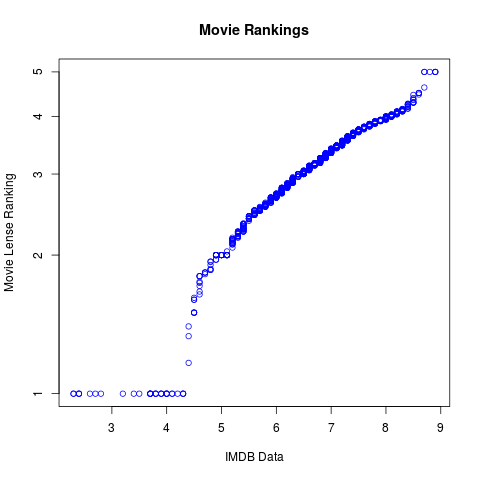
\includegraphics[scale=0.85]{Graph}
\caption{Movie Rankings}
\label{overflow}
\end{figure}


\end{answer}
\newpage 
\printbibliography
\end{document}